
\subsection{Probleme von FastTrack}
\label{subsec:probT}

Eines der Probleme die aus dem Messungen, wie in Abbildung \ref{fig:rtt} zu erkennen ist, das die Round Trip Time von etwa 85 \% der SNs bei maximal 100 ms beträgt.
Wie in der Abbildung \ref{fig:rttcaida} von Caida.org von 2001 \cite{caida} zu erkennen, dass die RTT von Amerika nach Europa und Asien etwa 200 ms beträgt.
Somit wird es schwierig das ganze Netzwerk zu durchsuchen, da nicht alle SNs erreicht werden.

\begin{figure}
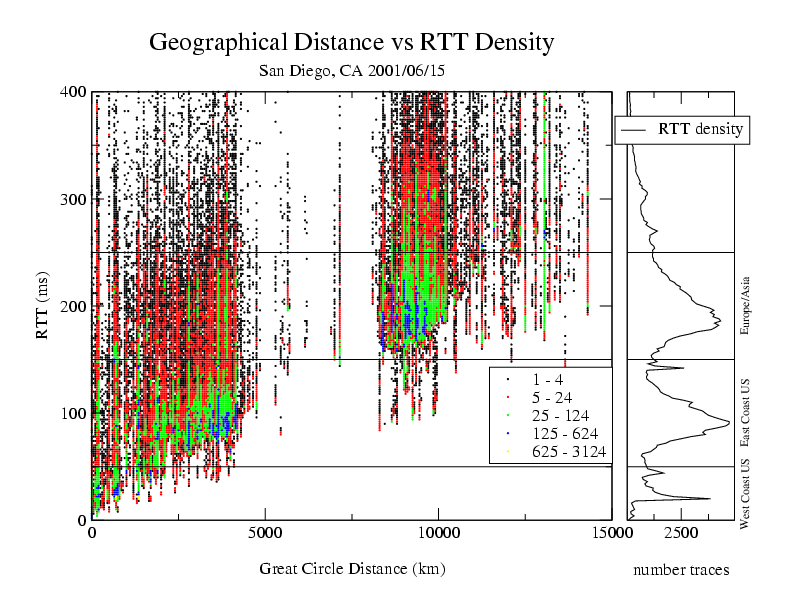
\includegraphics[scale=0.3]{gfx/dist_density_rie_20010513}
\caption{RTT Messung von Caida (Quelle \cite{caida})}
\label{fig:rttcaida}
\end{figure}


\subsubsection{UHASH}
\label{subsubsec:uhash}

Ein weiteres Problem ist der Content Hash Funktion UUHash \cite{uuHash} von FastTrack.
Der Hash wird schnell berechnet, da alle $2^n, n \in \mathbb{N}$ nur 300 KiB in die Berechnung einfließen.
Somit ist es möglich die Bereiche, welche nicht zur Hash Berechnung verwendet wurde mit Schadcode zu füllen.
Dies führte jedoch auch zu einem Problem, so das 2005 etwa 50\% aller Dateien infiziert waren. \cite{menneck2} 


\subsection{Implementationen}
\label{subsec:impl}

Die offizielle Implementierung des FastTrack Netzwerkes ist Kazaa \cite{kazaa} von den Beiden FastTrack Entwicklern.

Eine verbreitete inoffizielle Implementierung ist die Kazaa-Lite \cite{kazaaLite} Version.
Diese verwendet bei der Suche nicht nur den Eltern SN sondern versucht an mehrere SNs seine Suchanfrage zu senden und schließt die Verbindung nach der Antwort wieder\cite{liang2006fasttrack}.

Zwei andere Implementierungen, welche das FastTrack Netwerk benutzten sind Grokster \cite{grokster} und Morpheus \cite{morpheus}, wobei Morpheus 2002 auf das Gnutella \cite{gnutella} Netzwerk umgestiegen ist. \cite{morphvsKazaa}

Außerdem gibt es eine Implementierung für giFT \cite{gift}, dies ist eine Sammlung für Peer-To-Peer Protokolle und FastTrack wurde per reverse Engineering als Plugin hinzugefügt \cite{liang2006fasttrack}

Eine der bekanntesten Weiterentwicklung die auf FastTrack basiert und aufbaut ist Skype \cite{skypeAna}, welches von den selben Entwicklern entwickelt wurde.